\documentclass{beamer}

\mode<presentation>{
\definecolor{cured}{rgb}{.8,0,.2}
\usecolortheme[named=cured]{structure}
\usetheme{split}
}

\usepackage{amsopn}

\DeclareMathOperator{\conv}{conv}
\DeclareMathOperator{\average}{average}
\DeclareMathOperator{\support}{support}
\DeclareMathOperator{\boundary}{\partial}

 
%\usepackage{amsthm}

\newcommand{\centeripe}[1]{\begin{center}\Ipe{#1}\end{center}}
\newcommand{\comment}[1]{}

\newcommand{\centerpsfig}[1]{\centerline{\psfig{#1}}}

\newcommand{\seclabel}[1]{\label{sec:#1}}
\newcommand{\Secref}[1]{Section~\ref{sec:#1}}
\newcommand{\secref}[1]{\mbox{Section~\ref{sec:#1}}}

\newcommand{\alglabel}[1]{\label{alg:#1}}
\newcommand{\Algref}[1]{Algorithm~\ref{alg:#1}}
\newcommand{\algref}[1]{\mbox{Algorithm~\ref{alg:#1}}}

\newcommand{\applabel}[1]{\label{app:#1}}
\newcommand{\Appref}[1]{Appendix~\ref{app:#1}}
\newcommand{\appref}[1]{\mbox{Appendix~\ref{app:#1}}}

\newcommand{\tablabel}[1]{\label{tab:#1}}
\newcommand{\Tabref}[1]{Table~\ref{tab:#1}}
\newcommand{\tabref}[1]{Table~\ref{tab:#1}}

\newcommand{\figlabel}[1]{\label{fig:#1}}
\newcommand{\Figref}[1]{Figure~\ref{fig:#1}}
\newcommand{\figref}[1]{\mbox{Figure~\ref{fig:#1}}}

\newcommand{\eqlabel}[1]{\label{eq:#1}}
\newcommand{\eqref}[1]{(\ref{eq:#1})}

\newtheorem{thm}{Theorem}{\bfseries}{\itshape}
\newcommand{\thmlabel}[1]{\label{thm:#1}}
\newcommand{\thmref}[1]{Theorem~\ref{thm:#1}}

\newtheorem{lem}{Lemma}{\bfseries}{\itshape}
\newcommand{\lemlabel}[1]{\label{lem:#1}}
\newcommand{\lemref}[1]{Lemma~\ref{lem:#1}}

\newtheorem{cor}{Corollary}{\bfseries}{\itshape}
\newcommand{\corlabel}[1]{\label{cor:#1}}
\newcommand{\corref}[1]{Corollary~\ref{cor:#1}}

\newtheorem{obs}{Observation}{\bfseries}{\itshape}
\newcommand{\obslabel}[1]{\label{obs:#1}}
\newcommand{\obsref}[1]{Observation~\ref{obs:#1}}

\newtheorem{assumption}{Assumption}{\bfseries}{\rm}
\newenvironment{ass}{\begin{assumption}\rm}{\end{assumption}}
\newcommand{\asslabel}[1]{\label{ass:#1}}
\newcommand{\assref}[1]{Assumption~\ref{ass:#1}}

\newcommand{\proclabel}[1]{\label{alg:#1}}
\newcommand{\procref}[1]{Procedure~\ref{alg:#1}}

\newtheorem{rem}{Remark}
\newtheorem{op}{Open Problem}

\newcommand{\etal}{\emph{et al}}

\newcommand{\voronoi}{Vorono\u\i}
\newcommand{\ceil}[1]{\left\lceil #1 \right\rceil}
\newcommand{\floor}[1]{\left\lfloor #1 \right\rfloor}



\newcommand{\pin}{p_{\mathsf{in}}}
\newcommand{\pout}{p_{\mathsf{out}}}
\DeclareMathOperator{\cost}{cost}
\DeclareMathOperator{\depth}{depth}

\title{Distribution-Sensitive Point Location\\ in Convex Subdivisions}
\author{Pat Morin}
\institute{Carleton University}
\date{December 6, 2006 \\ McGill University}

\begin{document}

\frame{\titlepage}

\section[Outline]{}
\frame{\tableofcontents}

\section{Introduction}
\subsection{Planar Point Location}
\frame
{
  \frametitle{Planar Point Location}
  \begin{itemize}
  \item Preprocess a planar subdivision $G$ so that, for any query
point $p\in\R^2$, the we can quickly determine the face of $G$
that contains $p$
  \begin{center}
  \only<1>{\includegraphics{pl-1}}%
  \only<2>{\includegraphics{pl-2}}%
  \only<3>{\includegraphics{pl-3}}%
  \end{center}
  \end{itemize}
}

\subsection{History}

\frame
{
  \frametitle{The 1980s}
  \begin{itemize}
  \item<1-> After a few initial attempts, optimal $O(n)$ space, $O(\log
n)$ query time solutions were obtained by
  \begin{itemize}
   \item<2-> Kirkpatrick (1983) --- Independent set removal
   \item<3-> Edelsbrunner, Guibas, and Stolfi (1986) --- Fractional cascading
   \item<4-> Sarnak and Tarjan (1986) --- Persistence
   \item<5-> Mulmuley (1990) --- Randomized incremental construction
  \end{itemize}
  \end{itemize}
}

\frame
{
  \frametitle{The 1990s}
  \begin{itemize}
  \item<1-> Then we started carefully studying the constants:
   \item<2-> Goodrich, Orletsky, and Ramaiyer (1997)
   \begin{itemize}
      \item<3-> $O(n)$ space, $2\log n + o(\log n)$ standard comparisons
      \item<4-> Conjectured that $2\log n$ is optimal for linear space structures
   \end{itemize}
   \item<5-> Adamy and Seidel (1998)
   \begin{itemize}
      \item<6-> $O(n)$ space, $\log n + \sqrt{2}\log\log n +
o(\log\log n)$ standard comparisons
      \item<7-> Optimal up to the second term
   \end{itemize}
  \end{itemize}
}

\frame
{
  \frametitle{The New Millenium --- A New Era of Sensitivity}
  \begin{itemize}
  \item<1-> Adamy and Seidel's result closes the problem of the
	worst-case complexity of planar point location
  \item<2-> What about the average case?
  \item<3-> Assume the point $p$ is selected according to a
	probability measure $D$ over $\R^2$
  \item<4-> Given $(G,D)$ can we optimize the expected cost of
	locating $p$?
  \end{itemize}
}

\frame
{
  \frametitle{Defining Optimality}
  \begin{itemize}
   \item<1-> We need a way of knowing when a point location structure
	is optimal
   \item<2-> $D$ induces a distribution over the faces of $G$
   \item<3-> Let $p_i=\Pr\{\mbox{$p$ is contained in face $i$}\}$
   \item<4-> \textbf{Theorem (Shannon 1948):}
     For any data structure $X$ that makes only binary decisions, the
expected number of decisions is at least
   \[
      \mu_D(X) \ge H(p_1,\ldots,p_f) = \sum_{i=1}^f p_i\log(1/p_i)  \enspace .
   \]
  \end{itemize}
}

\frame
{
   \frametitle{Distribution-Sensitive Point Location: Results}
   \begin{itemize}
   \item<1-> Arya, Cheng, Mount, and Ramesh (2000)
    \begin{itemize}
      \item<1->For convex subdivisions: $O(n^2)$ space, $2H+o(H)$ comparisons
      \item<1->For convex subdivisions: $O(n)$ space, $4H+o(H)$ comparisons
      \item<1->Requires that $x$ and $y$ coordinates of $p$ are independent
    \end{itemize}
   \item<2-> Arya, Malamatos, and Mount (2000)
    \begin{itemize}
      \item<2->For triangulations: $O(n\log n)$ space, $H+o(H)$ comparisons
    \end{itemize} 
    \item<3-> Arya, Malamatos, and Mount (2001a)
    \begin{itemize}
      \item<3->For triangulations: $O(n\log^* n)$ space, $H+o(H)$ comparisons
    \end{itemize} 
    \item<4-> Arya, Malamatos, and Mount (2001b)
    \begin{itemize}
      \item<4->For triangulations: $O(n)$ space, $O(H)$ comparisons (randomized)
    \end{itemize} 
    \item<5-> Iacono (2001)
    \begin{itemize}
      \item<5->For triangulations: $O(n)$ space, $O(H)$ comparisons (deterministic)
    \end{itemize} 
   \end{itemize}


}

\section{Point-in-Polygon Testing}
\frame
{
   \frametitle{Point-in-Polygon Testing}
   \begin{itemize}
   \item<1-> It looks like distribution-sensitive point location is 
	well understood, but\ldots
   \item<2-> A simple question: $P$ is a convex $n$-gon, $D$ is a
	probability measure over $\R^2$
   \item<3-> Preprocess $(P,D)$ so that we can quickly determine if a
point $p$, distributed according to $D$ is inside or outside $P$
   \item<4-> None of the above results apply
   \end{itemize}
}

\frame
{
   \frametitle{Difficulties I}
   \begin{itemize}
   \item<1-> We will want to prove that our data structure is optimal
   \item<2-> But there are only two outcomes, so
     \[ H= \pin\log (1/\pin) + \pout\log(1/\pout) \le 1  \]
   \item<3-> We can't always match the entropy lower bound!
   \end{itemize}
}

\frame
{
   \frametitle{Difficulties}
   \begin{itemize}
     \item<1-> We could try to triangulate $P$ and apply a result for 
	triangulations\\
     \only<1>{\centerline{\includegraphics[scale=.6]{problema-1}}%
        -}       
     \only<2>{\centerline{\includegraphics[scale=.6]{problema-2}}%
        $H= \sum_{i=1}^f (c/f)\log (f/c) = \Theta(\log f)$ }%       
     \only<3->{\centerline{\includegraphics[scale=.6]{problema-3}}%
        $H= p_1\sum_{i=1}^3 p_i\log(1/p_i) = O(1)$ }%  
     \item<4-> Choosing correct triangulation is critical
   \end{itemize}
}

\subsection{The Triangle Tree}
\frame
{
   \frametitle{The Triangle Tree}
   \begin{itemize}
    \item<1-> We define a binary \emph{triangle tree} $T=T(P,D)$
    \item<2-> The vertices of $T$ correspond to triangles
    \item<3-> Each triangle approximates a section of the boundary of $P$
    {\includegraphics{ssplit-a}}
    \only<4>{\includegraphics{ssplit-b}}%
    \only<5>{\includegraphics{ssplit-c}}%
    \only<6>{\includegraphics{ssplit-d}}%
    \only<7->{\includegraphics{ssplit-e}}%
    \item<4-> Each internal node is split into two triangles
    \item<8-> The leaves of $T$ correspond to triangles completely
	contained in $P$
   \end{itemize}
}

\frame
{
   \frametitle{The Triangle Tree (Example)}
   \only<1>{\includegraphics{construction-d}}%
   \only<2>{\includegraphics{construction-e}}%
   \only<3>{\includegraphics{construction-f}}%
   \only<4>{\includegraphics{construction-g}}\\
}


\frame
{
   \frametitle{Searching in $T$}
   \begin{itemize}
     \item<1-> Searching in $T$ is done top-down, starting at the root
     \item<2-> For each triangle either:
      \begin{itemize}
        \item<3-> We finish the search:\\
          \includegraphics{finish}
        \item<4-> We recurse on one of the two children:\\
          \includegraphics{recurse}
      \end{itemize}
   \end{itemize}
}

\subsection{The Upper Bound}
\frame
{
   \frametitle{Analysis of the Triangle Tree}
   \begin{itemize}
   \item<1-> Let $\Pr(v)$ denote the probability that a search for $p$ 
	finishes at node $v\in T$
   \item<2-> Note that, if $v$ is at depth $i$ in $T$ then $\Pr(v)\le 1/2^i$
   \item<3-> So, the expected cost of searching in $T$ is at most
   \begin{eqnarray*}
      \mu_D(T) 
    &=& O(1) + O(1)\times\sum_{v\in T} \Pr(v)\times\depth(v) \\
       &\le& O(1)+O(1)\times \sum_{v\in T} \Pr(v)\log(1/\Pr(v))
   \end{eqnarray*}
   \end{itemize}

}

\frame
{
	\frametitle{Review and Lookahead}
	\begin{itemize}
	\item<1-> We have a triangle tree $T$ whose search time is
	 \[ \mu_D(T) \le O(1)+O(1)\times \sum_{v\in T} \Pr(v)\log(1/\Pr(v))
         \]
	and we want to show that this is optimal 
        \item<2-> We will show that every point location structure $X$ for
	$P$ is also a point location structure for the triangles of
$T$, so Shannon's Theorem gives
	 \[ \mu_D(X) \ge \sum_{v\in T} \Pr(v)\log(1/\Pr(v))
         \]
        \item<3-> Well, not exactly\ldots
          \begin{itemize}
		\item<4-> $X$ can distinguish between most (but not all) triangles of $T$
		\item<5-> But this will be good enough
          \end{itemize}
	\end{itemize}
}

\subsection{The Lower Bound}
\frame
{
   \frametitle{Linear Decision Trees}
   \begin{itemize}
     \item<1-> We need to fix a model of computation for the lower bound
     \item<2-> A \emph{linear decision tree} is a binary where
       \begin{itemize}
          \item Each internal node is labelled with a linear inequality
          \item Each leaf is labelled with \emph{in} or \emph{out}
          \item For every $p\in\R^2$ the search path for $p$ finishes at 
           a leaf labelled \emph{in} if and only if $p\in P$
       \end{itemize}
     \item<3-> Every point location structure in the
	introduction can be expressed as a linear decision tree
   \end{itemize}
}

\frame
{
	\frametitle{Linear Decision Tree Example}
        \only<1>{\includegraphics{ld-a}}%
        \only<2>{\includegraphics{ld-b}}%
        \only<3>{\includegraphics{ld-c}}%
        \only<4>{\includegraphics{ld-d}}%
        \only<5>{\includegraphics{ld-e}}%
}


\frame
{
	\frametitle{A Non-Trivial Lower Bound}
        \begin{itemize}
          \item<1-> Suppose we have this polygon $P$ and this distribution $D$:
            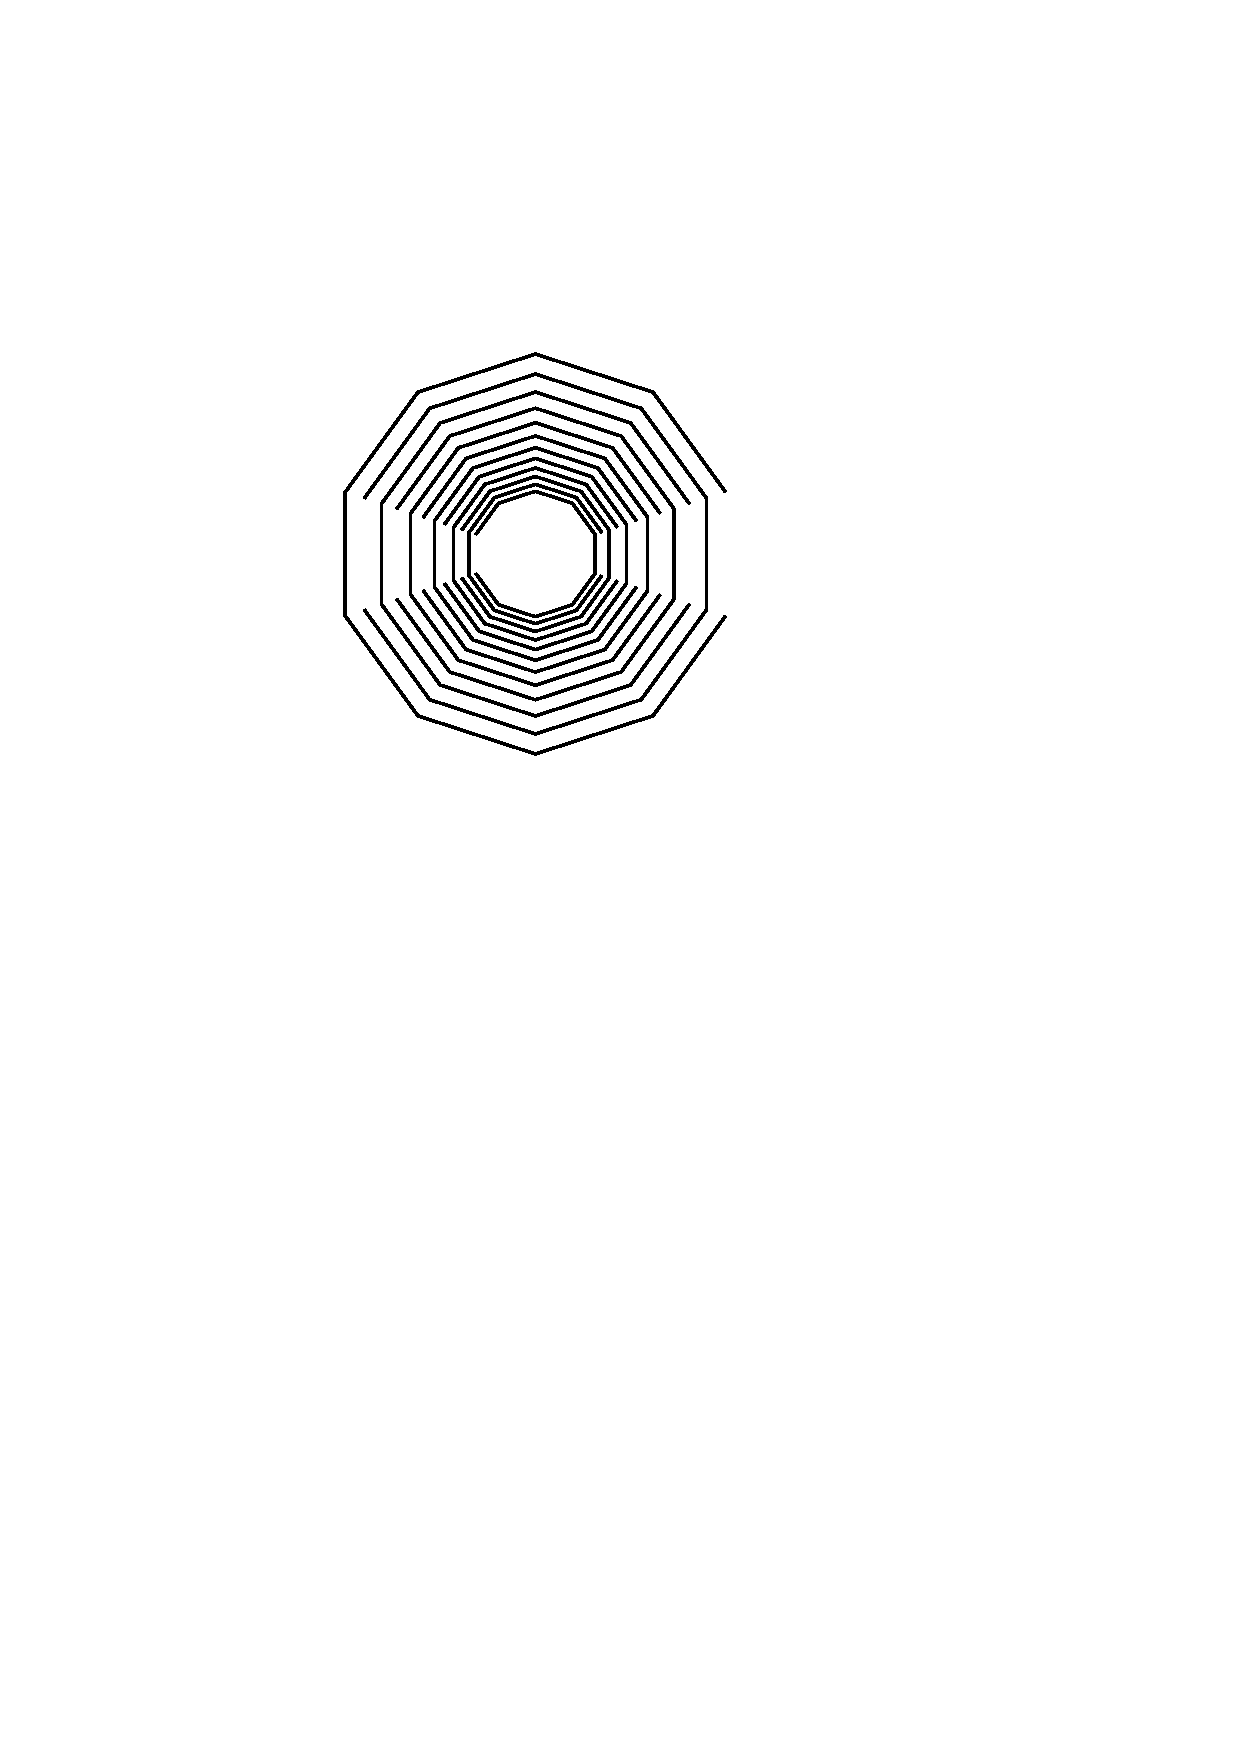
\includegraphics{lower-bound}
          \item<2-> \textbf{Lemma 0:} Any linear decision tree $X$ for
testing if $p\in P$ has 
\[  \mu_D(X)\ge \frac{1}{2}\sum_{i=1}^{11} p_i\log(1/p_i)  \]
        \end{itemize} 
}


\frame
{
	\frametitle{Proof of Lemma 0}
        \begin{itemize}
           \item<1->We first prove a lower bound for the \emph{chord tree} model\\
            \only<1>{\includegraphics{lb-proof-a}}%
            \only<2>{\includegraphics{lb-proof-b}}%
            \only<3>{\includegraphics{lb-proof-c}}%
            \only<4->{\includegraphics{lb-proof-d}}%
           \item<2->Let $C_1,\ldots,C_{11}$ be the components of 
               $\support(D)\setminus \boundary P$

           \item<3->For any $p\in C_i$ and $q\in C_j$ $i\neq j$, $p$ and $q$
               must live in different leaves of the chord tree

           \item<4->By labelling leaves of the chord tree $T_C$
		appropriately we obtain a
               point location structure for $C_1,\ldots,C_{11}$ \\
           $\Rightarrow$ By Shannon's Theorem $\mu_D(T_C) \ge \sum_{i=1}^{11}p_i\log (1/p_i)$
           \item<5->Any line intersects $\support(D)$ in at most 2 chords
		\hfill{\qed}
        \end{itemize}
}


\frame
{
    \frametitle{Using Lemma 0}
    \begin{itemize}
	\item<1-> Let $V\subseteq V(T)$ be such that no vertex in
$V$ is an ancestor of any other vertex in $V$
        \item<2-> The triangles of $V$ look like this:\\
	\includegraphics{using-lemma0}
        \item<3->Let $D_{\mid V}$ be the measure $D$ conditioned on the
search completing at a node in $V$
        \item<4->\textbf{Lemma 1:} For any linear decision tree $X$
        \[ \mu_{D_{\mid V}}(X) \ge \frac{1}{4}\sum_{v\in V} \Pr(v\mid V)\log (1/\Pr(v\mid V))
         \]
    \end{itemize}
}

\frame{
     \frametitle{Review}

     \begin{itemize}
	\item<1-> We have a triangle tree $T$ whose search time is
	 \[ \mu_D(T) \le O(1)+O(1)\times \sum_{v\in T} \Pr(v)\log(1/\Pr(v))
         \]
        \item<2-> For any linear decision tree $X$ and any
	\emph{genetically independent set} $V\subseteq V(T)$ of
	 \[ \mu_{D_{\mid V}}(X) \ge \frac{1}{4}\sum_{v\in V} \Pr(v\mid V)\log(1/\Pr(v\mid V))
         \]
        \item<3-> For any partition of $V(T)$ into genetically
independent sets $V_1,\ldots,V_k$, and any linear decision tree $X$,
	 \[ \mu_D(X) \ge \frac{1}{4}\sum_{i=1}^k\Pr(V_i)\sum_{v\in V_i} \Pr(v\mid
V_i)\log(1/\Pr(v\mid V_i))
         \]
     \end{itemize}
}


\frame
{
	\frametitle{Review (Cont'd)}

 	\begin{itemize}
	\item<1-> We're now dangerously close to matching upper and lower bounds
        \begin{eqnarray*}
	\mu_D(X) &\ge &\frac{1}{4}\sum_{i=1}^k
	   \Pr(V_i)\sum_{v\in V_i} \Pr(v\mid V_i)\log(1/\Pr(v\mid V_i)) \\
	& = &\frac{1}{4}\sum_{i=1}^k\sum_{v\in V_i} 
		\Pr(v)\log(1/\Pr(v\mid V_i)) \\
	& = &\frac{1}{4}\sum_{i=1}^k\sum_{v\in V_i} 
		\Pr(v)(\log(1/\Pr(v))-\log(1/\Pr(V_i)))
	\end{eqnarray*}
	\item<2-> The trick is to pick our $V_i$s so that
$\log(1/\Pr(V_i))$ is small
	\end{itemize}

}


\frame
{
	\frametitle{Picking the $V_i$s}

	\begin{itemize}
	\item<1-> Let
	\[
		V_i=\{v\in V(T) :1/2^{i-1} \le \Pr(v) \le 1/2^i \}
	\]
	\item<2-> But these $V_i$ are not genetically independent!
 	\item<3-> While $|V_i|\ge 2^{\alpha i}$  [constant $0< \alpha
< 1$]
	   \begin{itemize}
		\item $V_{i,j}$ is a genetically independent subset of
			$V_i$ with size $2^{\alpha i}/i$
		\item $V_i\gets V_i\setminus V_{i,j}$
		\item $j\gets j+1$
	   \end{itemize}
	\item<4-> With the right $\alpha$ and some work, we can show that
	\begin{eqnarray*}
	\mu_D(X) & \ge & \frac{1}{4}\sum_{i,j}\sum_{v\in V_{i,j}} 
		\Pr(v)(\log(1/\Pr(v))-\log(1/\Pr(V_{i,j}))) \\
	& \ge & \left(\frac{1}{4}-\epsilon\right)\sum_{v\in T}\Pr(V)\log(1/\Pr(V)) -
O(1)
	\end{eqnarray*}
	\end{itemize}
}

\frame
{
	\frametitle{Theorem 1}
	\begin{itemize}
	\item<1-> For any convex $n$-gon $P$ and
any probability measure $D$ over $\R^2$, a triangle tree $T=T(P,D)$ can be
constructed in $O(n)$ time and 
\[
	\mu_D(T) = O(1) + O(1)\times\sum_{v\in V(T)} \Pr(v)\log(1/\Pr(v))
\enspace .
\]

	\item<2-> Furthermore, for any linear decision tree $X$ that
	tests if a point $p$ is contained in $P$,
	\[
	\mu_D(X) = \Omega(1) + \Omega(1)\times\sum_{v\in V(T)}
	\Pr(v)\log(1/\Pr(v)) \enspace .
	\]
	\end{itemize}
}


\section{Point Location in Convex Subdivisions}
\frame
{
	\frametitle{Point Location in Convex Subdivisions}

	\begin{itemize}
	\item<1-> Given a convex subdivision $G$ having faces
$F_1,\ldots,F_f$ and a probability measure $D$ over $\R^2$

	\item<2-> For each $i$, triangulate $F_i$ using the triangles of
the triangle tree $T_i=T(F_i,D_{\mid F_i})$

	\item<3-> Preprocess the resulting triangulation using Iacono's
distribution-sensitive point location structure for triangulations to
obtain a data structure $Q$

	\end{itemize}
}

\frame
{
	\frametitle{Analysis of $Q$}

	\begin{eqnarray*}
	\mu_D(Q) & = & O(1)+O(1)\times\sum_{i=1}^f\sum_{v\in
T_i}\Pr(v)\log(1/\Pr(v)) \\
	         & = & O(1) \\ & & {}+O(1)\times\sum_{i=1}^f\Pr(F_i)\log
(1/\Pr(F_i)) \\ & & {}+ O(1)\times\sum_{i=1}^f\Pr(F_i)\times\sum_{v\in T_i}\Pr(v\mid
F_i)\log(1/\Pr(v\mid F_i))
	\end{eqnarray*}
	\begin{itemize}
	\item<2->Each of these three terms is also a lower bound
	\end{itemize}
}

\frame
{
	\frametitle{Theorem 2}

	\begin{itemize}
	\item For any convex subdivision $G$ having complexity $n$ and
	any probability measure $D$ over $\R^2$, the data structure
$Q=Q(G,D)$ can be constructed in $O(n)$ time and 
	\begin{eqnarray*}
	\mu_D(Q) 
         & = & O(1)+O(1)\times\sum_{i=1}^f\Pr(F_i)\log
(1/\Pr(F_i)) \\ & & {}+ O(1)\times\sum_{i=1}^f\sum_{v\in T_i}\Pr(F_i)\Pr(v\mid
F_i)\log(1/\Pr(v\mid F_i))
	\end{eqnarray*}
	and this is (within a constant factor of) optimal in the linear decision tree model of
computation.
	\end{itemize}
}

\section{Summary and Conclusions}
\frame
{
	\frametitle{Summary and Conclusions}
	\textbf{Results:}
	\begin{itemize}
	\item<2-> A constant factor optimal data structure for
distributions-sensitive point location in convex subdivisions
	\end{itemize}
	\textbf{Open Problems:}
	\begin{itemize}
	\item<3-> The constant factor gap between the upper and lower
bounds is $4+\epsilon$.  Reduce this (to 1). 
	\item<4-> Obtain similar results for general (non-convex)
polygons and subdivisions
	\end{itemize}
}


\end{document}

